\documentclass[12pt, letterpaper, twoside]{report}
\usepackage[utf8]{inputenc}
\usepackage{amsmath}
\usepackage{mathtools}
\usepackage{graphicx}
\usepackage{subcaption}
\title{Programming Assignment2 }
\author{Prakhar Thakuria(EE16B061)}
\date { 15 February 2019}

\begin{document}

\maketitle
\section*{Question1}
\textbf{Solution:} \par
\section*{Puddle World}
1. There is a wall all around the the grid and if and action tries to go in the wall there is no change that is remains in the same state as before. 
 \begin{figure}[h!]
  \centering
    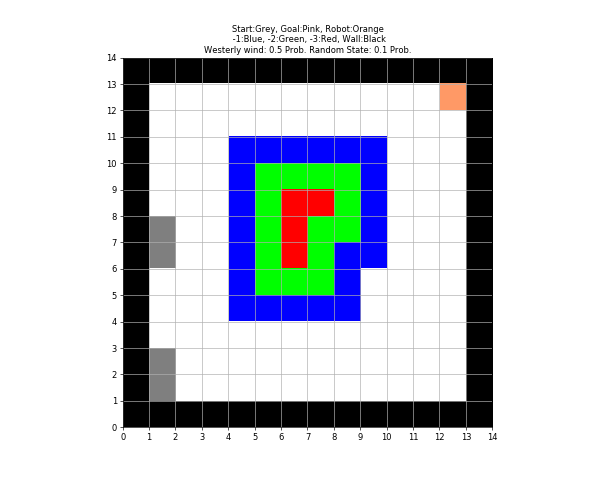
\includegraphics[width=0.8\linewidth]{Puddle.png}
  \caption{My Puddle World}
\end{figure}
 \newpage
 \textbf{Puddle}
\par
\begin{figure}[h!]
  \centering
  \begin{subfigure}[b]{0.7\linewidth}
    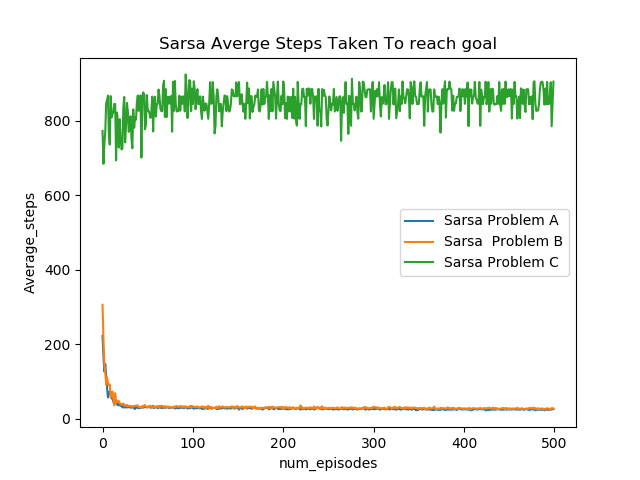
\includegraphics[width=\linewidth]{Sarsa_average_steps.png}
    \caption{Steps To Goal}
  \end{subfigure}
  \begin{subfigure}[b]{0.7\linewidth}
    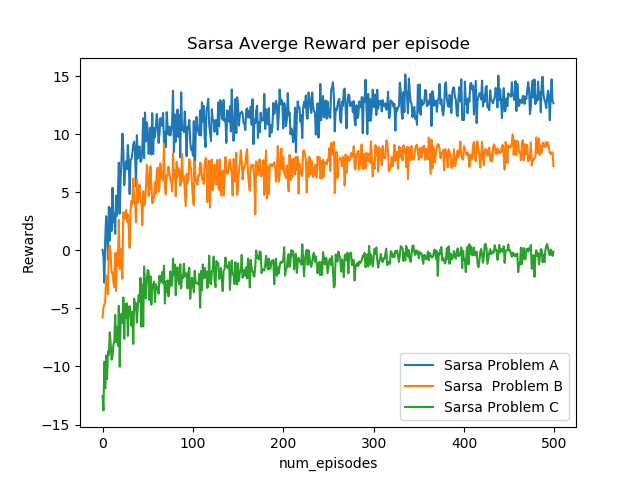
\includegraphics[width=\linewidth]{Sarsa_Total_Returns.png}
    \caption{Average Reward}
  \end{subfigure}
  \caption{Sarsa All Goals}
  \label{fig:Eps-Greedy}
\end{figure}
\begin{figure}[h!]
  \centering
    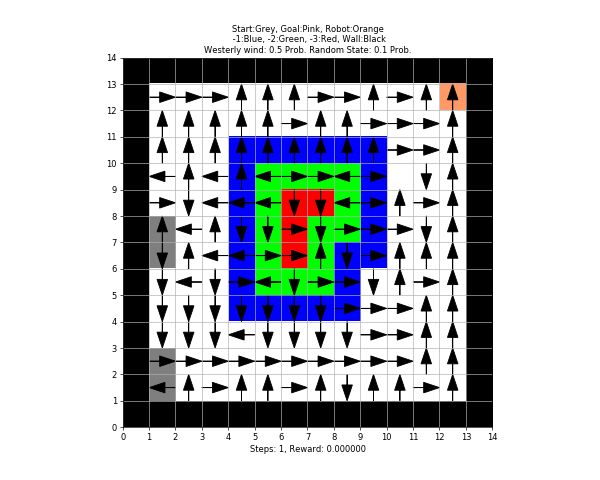
\includegraphics[width=0.8\linewidth]{Sarsa_Problem_A.png}
  \label{fig:Eps-Greedy}
\end{figure}
\begin{figure}[h!]
  \centering
    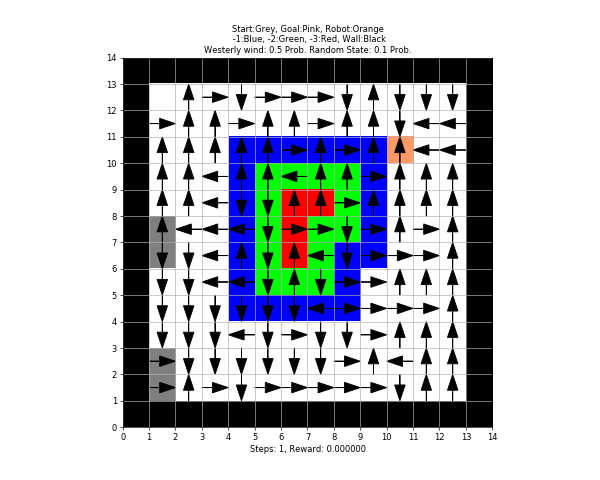
\includegraphics[width=0.8\linewidth]{Sarsa__Problem_B.png}
  \label{fig:Eps-Greedy}
\end{figure}
\begin{figure}[h!]
  \centering
    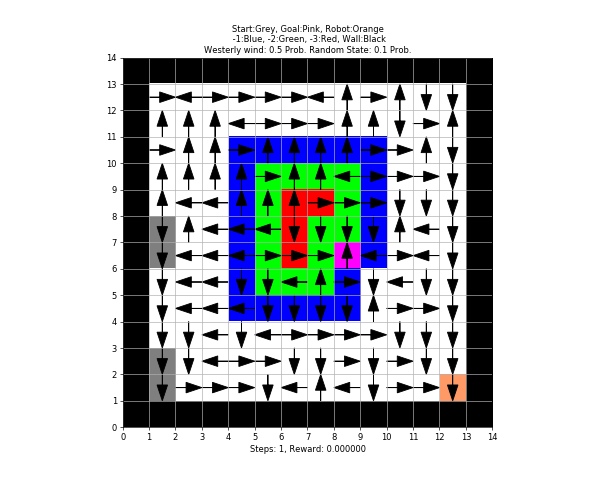
\includegraphics[width=0.8\linewidth]{Sarsa_Problem_C.png}
  \label{fig:Eps-Greedy}
\end{figure}
\newpage
\begin{figure}[h!]
  \centering
    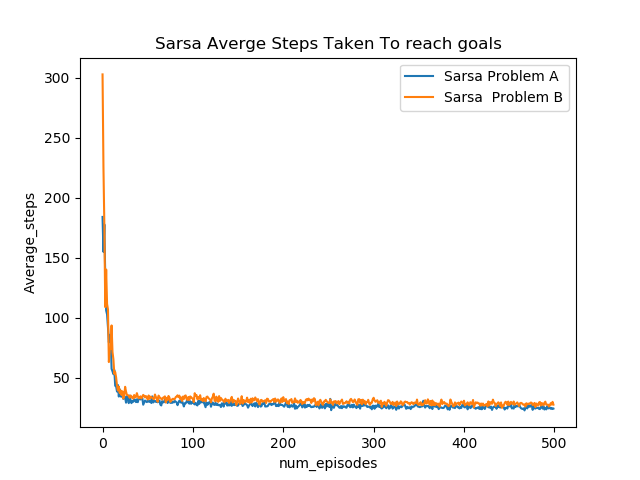
\includegraphics[width=\linewidth]{Sarsa_avg_steps.png}
  \label{fig:Eps-Greedy}
\end{figure}
\section*{Sarsa}
1. The update rule used was \newline
\[Q(S,A) = Q(S,A) + \alpha*(R + \gamma * Q(S',\pi(S') - Q(S,A)) \]
2. I made in a change for the last problem i.e. Goal == C that if does not reach the goal within 1000 steps, it truncates.
\section*{Observation}
1. It take a lot of time to reach the goal state in the case when goal is C it takes an average of over 10,000 steps to converge to the goal state while for others it is around 250.\par
This is due the fact Goal state C is covered by negative reward and hence if initialization 0 it tries to look at the possibilities before reaching the goal state.\newline
2. Since the goal state is A relatively far away from the puddle hence average reward is higher, while in the case of goal B as it is very near to the puddle the reward is relatively lower as it in the neighbourhood of the puddle. Similar explanation can be derived for goal state C \newline
3.For the optimal policy in the case A the puddle is , but in the case B also tries to move out of the puddle but to an extent it can also take one or two step in the puddle if ti take it closer to the goal through the puddle. but in the case of goal state C the optimal policies also go through the whole puddle for some states.\newline
4. As the the steps for goal states were not quite clear in the previous figure because of goal state C the above is a better view of the problem.
5. Since there is no negative rewards for the steps taken to reach goal it does not learn the shortest path to the goal.
\newpage
\section*{Question3}
\textbf{Solution:}\par
\par
\begin{figure}[h!]
  \centering
  \begin{subfigure}[b]{0.6\linewidth}
    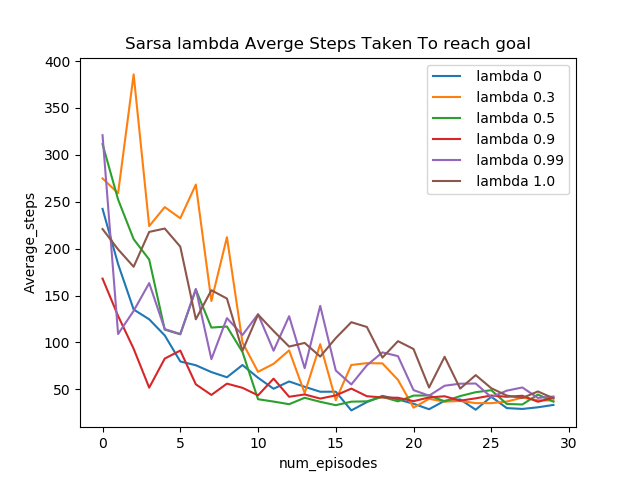
\includegraphics[width=\linewidth]{Sarasa_labda_goal_A_steps.png}
    \caption{Steps to Goal}
  \end{subfigure}
  \begin{subfigure}[b]{0.6\linewidth}
    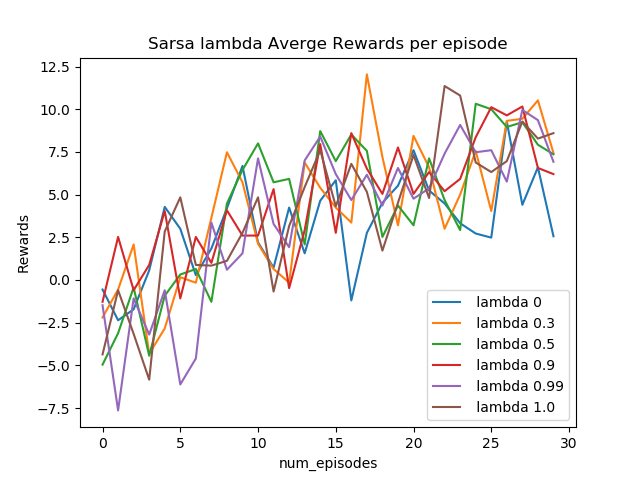
\includegraphics[width=\linewidth]{Sarasa_labda_goal_A_return.png}
    \caption{Average Reward}
  \end{subfigure}
  \caption{Sarsa Lambda goal A}
  \label{fig:Softamx}
\end{figure}
\begin{figure}[h!]
  \centering
  \begin{subfigure}[b]{0.6\linewidth}
    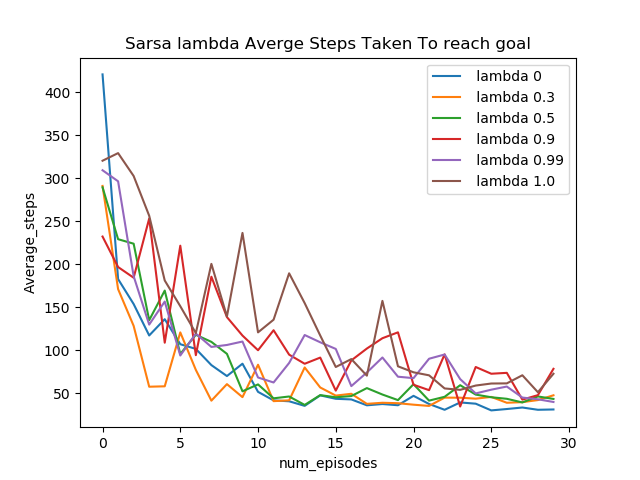
\includegraphics[width=\linewidth]{Sarasa_labda_goal_B_steps.png}
    \caption{Steps to Goal}
  \end{subfigure}
  \begin{subfigure}[b]{0.6\linewidth}
    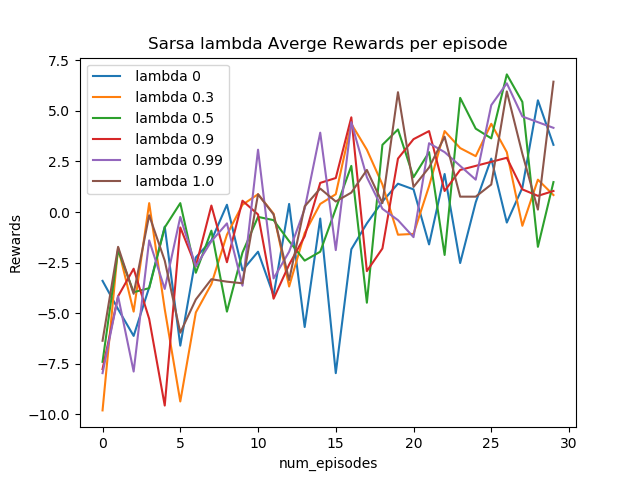
\includegraphics[width=\linewidth]{Sarasa_labda_goal_B_return.png}
    \caption{Average Rewards}
  \end{subfigure}
  \caption{Sarsa Lambda Goal B}
  \label{fig:Softamx}
\end{figure}
\begin{figure}[h!]
  \centering
  \begin{subfigure}[b]{0.6\linewidth}
    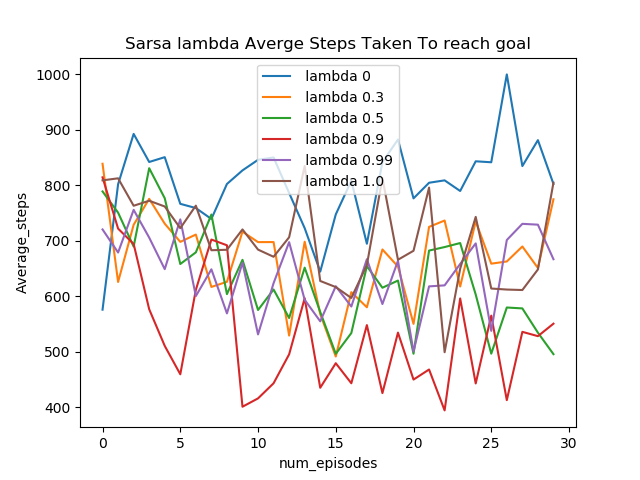
\includegraphics[width=\linewidth]{Sarasa_labda_goal_C_steps.png}
    \caption{Steps to Goal}
  \end{subfigure}
  \begin{subfigure}[b]{0.6\linewidth}
    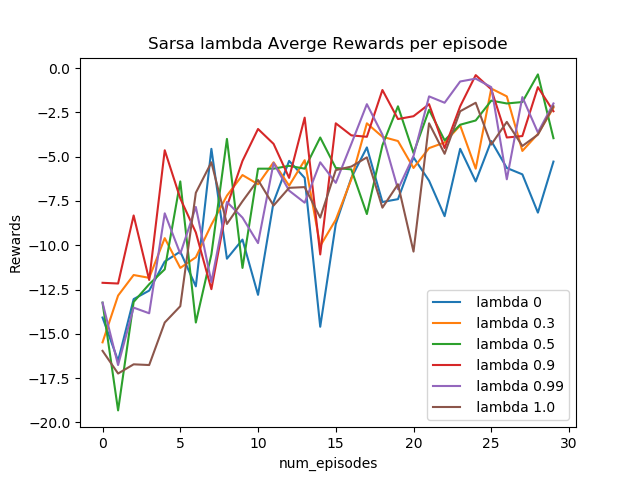
\includegraphics[width=\linewidth]{Sarasa_labda_goal_C_returns.png}
    \caption{Average Reward}
  \end{subfigure}
  \caption{Sarsa Lambda Goal C}
  \label{fig:Softamx}
\end{figure}
\textbf{Go to te last few pages to see the optimal policy for sarsa-lamda}
\section*{Sarsa($\lambda$)}

1. Used value of Lambda were: 0,0.3,0.5,0.9,0.99,.1.\newline
2. Accumulating traces were used for the development of the following graphs, as it  seemed to have a little less variance than replacing traces.\newline
3. There was a cap at of 1000 steps for termination.
\section*{Observation}
1. Sarsa Lambda takes a lot time to complete as the number of updates is lot more than the Sarsa and hence a lot less number of updates can be done and hence the all the possibilities are not explored. The number of iteration don't seem to be enough rather to make meaning full conclusions .\newline
2. For goal state == A, as the goal state is much far way from the puddle every lambda seems to be doing almost same. but in the case of goal state B returns tend to increase in the start and then decrease and lambda = 0.99 or 0.9 seams to have taken the lead but still the variance is just too much to say anything for sure.  \newline
3. Sarsa lambda takes care that the first step is i the right direction, which is not in the case of sarsa and the direction goes on for avoiding puddle as the lambda increases.(Refrence to last page where optimal policies are given)
3. There is a definite increase in the average reward in a lot less episodes than sarsa lambda over sarsa. What sarsa-lambda was able to achieve in 30 episodes sarsa took more than 100 episodes to do.\newline
4. Again the rewards as in the case for the goal C are very low but they increase as move along the episodes
5. Since there is no negative rewards for the steps taken to reach goal it does not learn the shortest path to the goal.
\section*{Question4}
\textbf{Solution:} \par
\section*{Learning parameters used}
 \[ \alpha  = .001 \gamma = 0.9\]
\begin{figure}[h!]
  \centering
  \begin{subfigure}[b]{0.6\linewidth}
    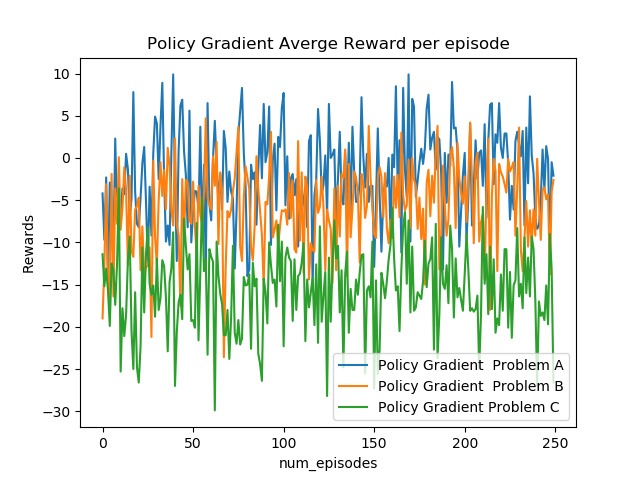
\includegraphics[width=\linewidth]{Policy_Gradient__rewards.png}
    \caption{Average Reward}
  \end{subfigure}
  \begin{subfigure}[b]{0.6\linewidth}
    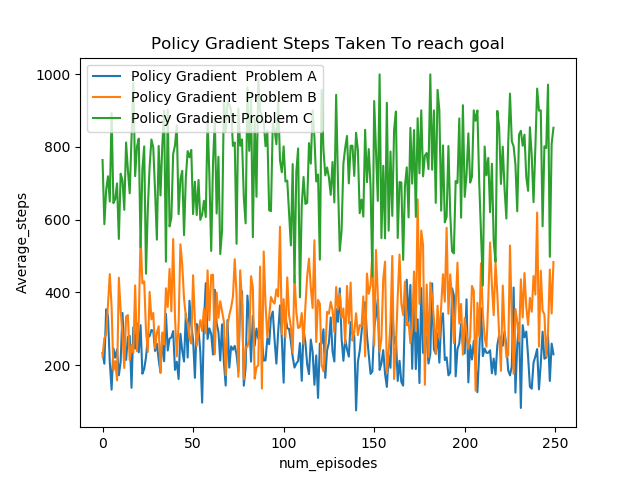
\includegraphics[width=\linewidth]{Policy_Gradient__steps.png}
    \caption{Steps To Goal}
  \end{subfigure}
  \caption{Policy Gradient all problems}
  \label{fig:Softamx}
\end{figure}
\section*{Policy Gradient Monte Carlo}
Since  Monte Carlo Policy Gradient uses episodes were generated and the limit was 1000 steps before that it the goal is not achieved then the the episode it terminated. And the  the iteration used were 10 , and episodes used were 250

\newpage
\begin{figure}[h!]
  \centering
  \begin{subfigure}[b]{0.5\linewidth}
    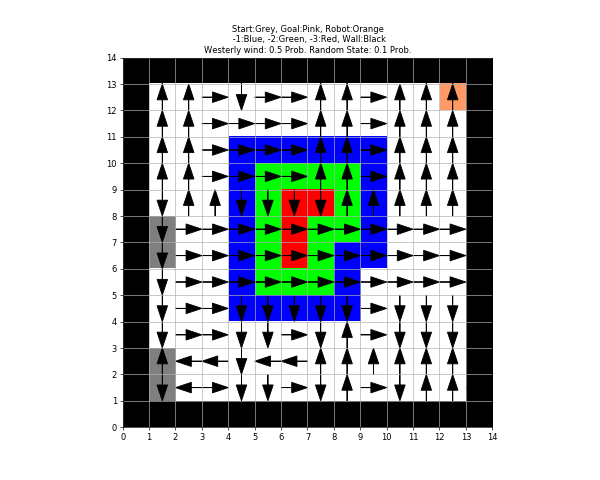
\includegraphics[width=0.8\linewidth]{Policy_Gradient__Problem_A_2.png}
    \caption{Problem A}
  \end{subfigure}
  \begin{subfigure}[b]{0.5\linewidth}
    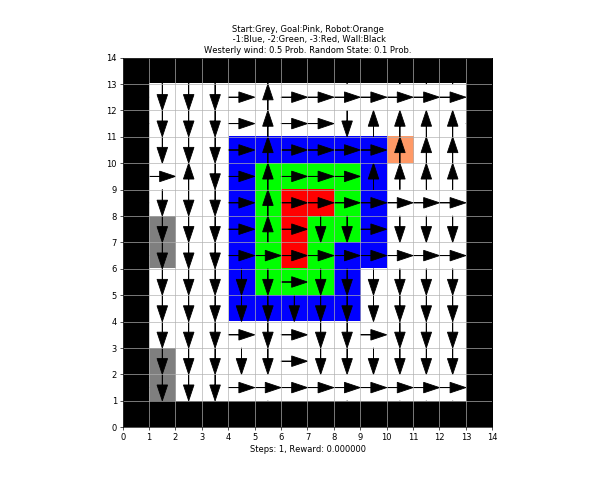
\includegraphics[width=0.8\linewidth]{Policy_Gradient__Problem_B.png}
    \caption{Problem B}
  \end{subfigure}
  \begin{subfigure}[b]{0.5\linewidth}
    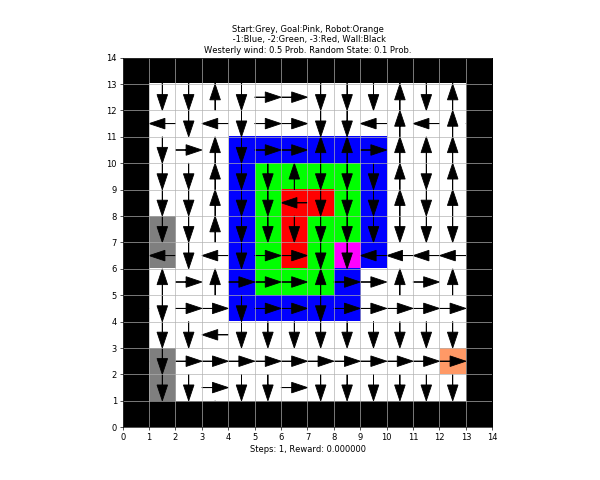
\includegraphics[width=0.8\linewidth]{Policy_Gradient_Problem_C.png}
    \caption{Problem C}
  \end{subfigure}
  \caption{Optimal Policies learnt $\alpha = 0.001 \gamma = 0.9$}
  \label{fig:Softamx}
\end{figure}
\newpage
\par
 \section*{Observation}
 1. In this case the average steps used for the terminating at the goal don't change that much as there is no compensation used for the number of steps in this case.\newline
 \[ \alpha  = .001 \gamma = 0.9\]
 2. The average reward increases a little bit although there is not much change(as compared to sarsa-lamda or even Sarsa). It still remains quite random, which just goes to show that it not a very good representation of the state space. This might be because the discount factor is to much and alpha is too low(As the number of iteration and episodes are limited we don't the luxury to use such a small alpha and gamma), hence I increased that for the next iteration.\newline
 \begin{figure}[h!]
  \centering
    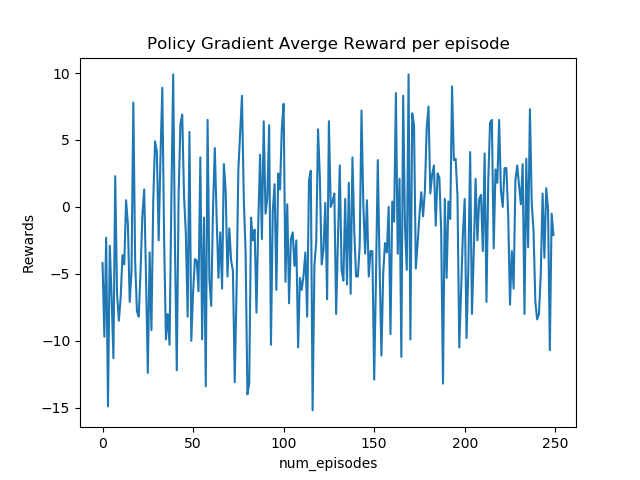
\includegraphics[width=0.5\linewidth]{Policy_Gradient_Averages_reward goal a.png}
  \caption{Policy Gradient Reward goal A}
\end{figure}
 \newpage
 
\[ \alpha = 0.1 \gamma = 0.99\] 
 \begin{figure}[h!]
  \centering
    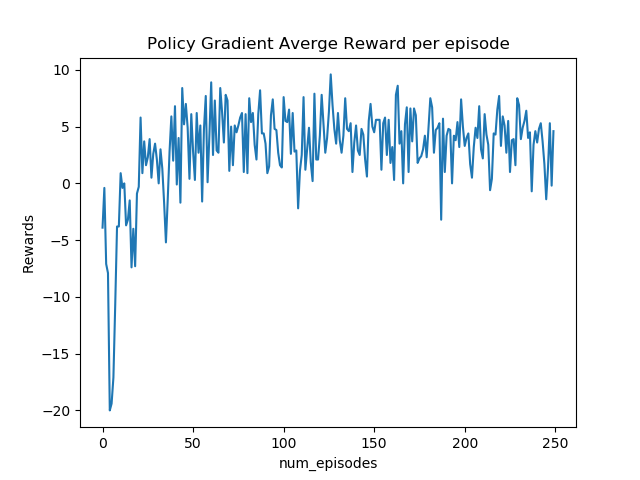
\includegraphics[width=0.5\linewidth]{Policy_Gradient_Averages_steps goal a.png}
  \caption{{Policy Gradient rewards A $\alpha = 0.1 \gamma = 0.99$}}
\end{figure}

3.This seems to be doing quite good even for the other cases as well as there is a constant increase in the reward but the the optimal policy learnt depend highly on the westerly wind in this case.\newline

4. As we can see the policy learnt for this is
\begin{figure}[h!]
  \centering
    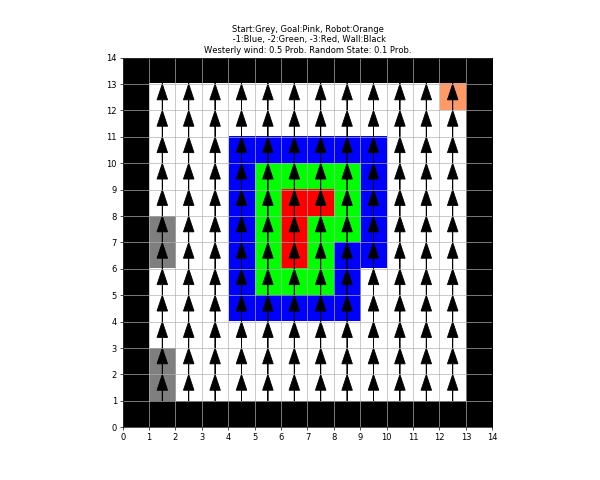
\includegraphics[width=0.5\linewidth]{Policy_Gradient__Problem_A.png}
  \caption{Optimal Policy Goal A $\alpha = 0.1 \gamma = 0.99$}
\end{figure}\newline
5. The complete picture for the parameters $\alpha = 0.1 and \gamma = 0.99$:
\begin{figure}[h!]
  \centering
    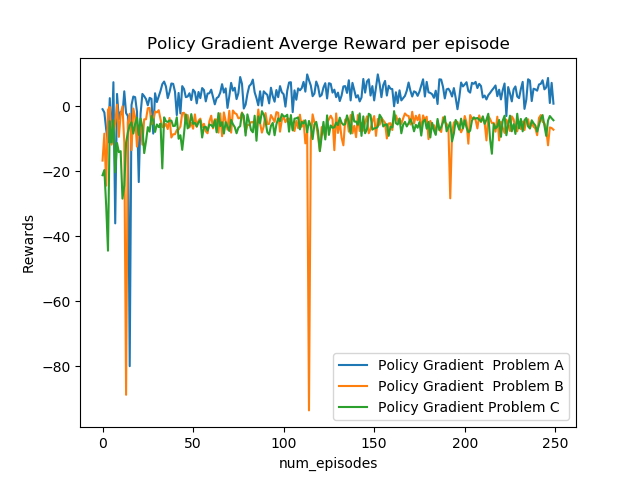
\includegraphics[width=0.5\linewidth]{jhblseriuglh.png}
  \caption{Average reward all goals $\alpha = 0.1 \gamma = 0.99$}
\end{figure}

\newpage
\section*{Question 5}
\textbf{Solution:} 

\textbf{Update Equations} 
 \[ \theta = \theta + \alpha \gamma G \Delta_\theta ln(\pi(A_t|S_t,\theta))\]
 For SoftMax
 \[ \Delta_\theta ln(\pi(A_t|S_t,\theta)) = 1 - \frac{1}{\Sigma(exp(\theta_x(x,a) +  \theta_y(y,a))}\]\
 As 
 \[ \pi(A_t|S_t,\theta) = \frac{exp(\theta_x(x,A_t) +  \theta_y(y,A_t))}{\Sigma(exp(\theta_x(x,a) +  \theta_y(y,a))} \]
\subsection*{Comments On the suitability}\par
1. For the given problem this is a not suitable at all as we can see we would get much better returns and much better policy in the with Sarsa. \newline
2. But in general it is quite use full to have such an parametrisation as it has limited number of parameters but still is able to have diff rent action probabilities in diff rent states. If the state space was to blow up we would not be able to maintain Q for all the state action pair and updating them would become even harder. Already given the episodes were less than 100 were not able to update all the state-action pairs. Hence, in such case the parametrization would help a lot if the states were to blow up.
\section*{Question6}
\textbf{Solution:} \par 
 No we won't be able to run the same code for the as the number of states hane now blown it won't be possible to run the same as the number of parameters have also grown exponentially.
 
 \section*{Results}
 This being time taking process i ran it for just Goal A  and the Average return results are:
 \begin{figure}[h!]
  \centering
  \begin{subfigure}[b]{0.5\linewidth}
    \includegraphics[width=0.5\linewidth]{Linear_approximation03_rewards.png}
    \caption{Steps to Goal}
  \end{subfigure}
  \begin{subfigure}[b]{0.5\linewidth}
    \includegraphics[width=0.5\linewidth]{Linear_approximation05_rewards.png}
    \caption{Average Rewards}
  \end{subfigure}
  \caption{Linear approximator}
  \label{fig:Softamx}
\end{figure}



\section*{Sarsa lamda optimal policy}

  \centering
  \begin{figure}[b]
    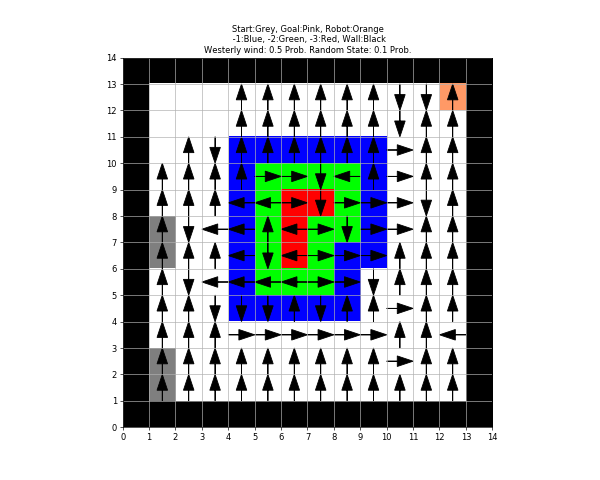
\includegraphics[width=\linewidth]{Sarsa_Problem_A_lambda_0.png}
    \caption{Sarsa lamnda(0) A }
  \end{figure}
  \centering
  \begin{figure}[b]
    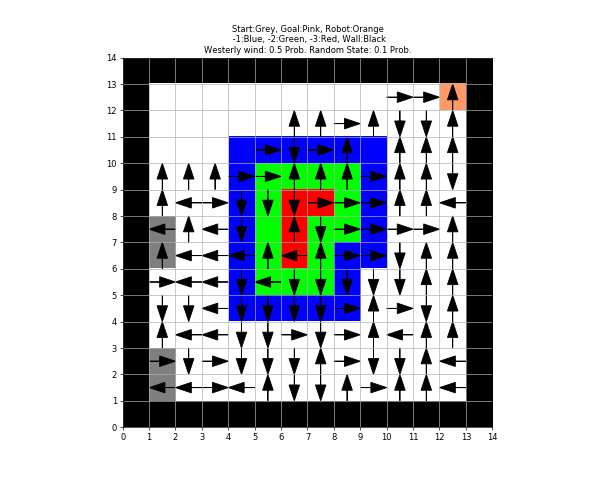
\includegraphics[width=\linewidth]{Sarsa_Problem_A_lambda_03.png}
    \caption{Sarsa lamnda(0.3) A}
  \end{figure}
  \centering
  \begin{figure}[b]
    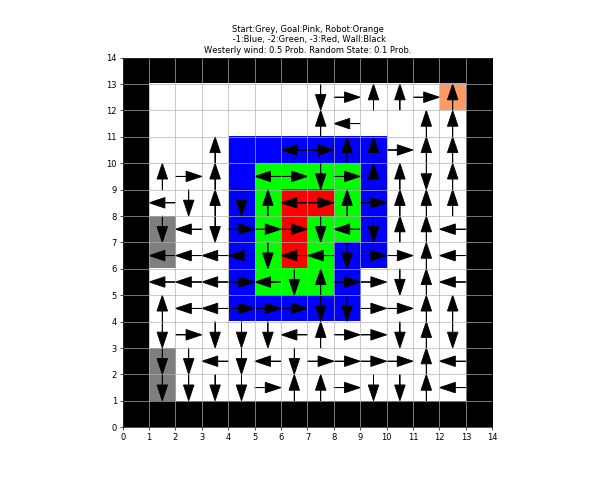
\includegraphics[width=\linewidth]{Sarsa_Problem_A_lambda_05.png}
    \caption{Sarsa lamnda(0.5) A}
  \end{figure}
  \newpage
  \centering
  \begin{figure}[b]
    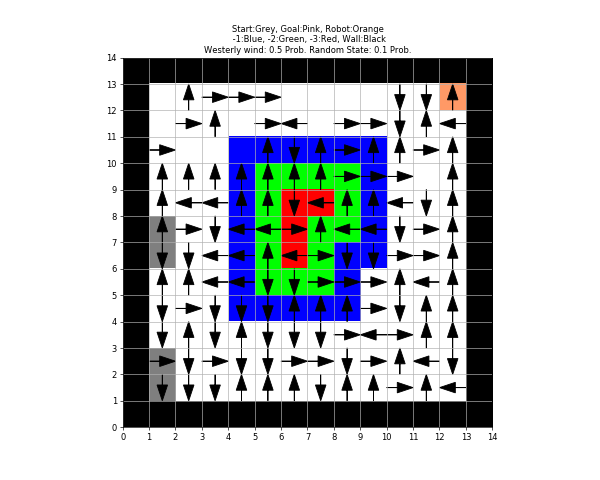
\includegraphics[width=\linewidth]{Sarsa_Problem_A_lambda_09.png}
    \caption{Sarsa lamnda(0.9) A}
  \end{figure}
  \begin{figure}[b]
    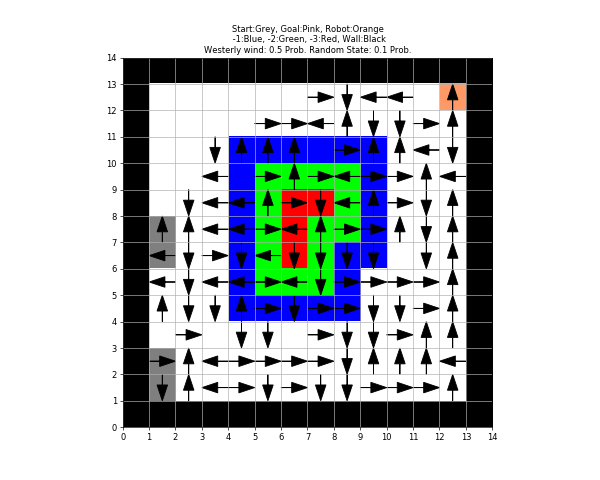
\includegraphics[width=\linewidth]{Sarsa_Problem_A_lambda_099.png}
    \caption{Sarsa lamnda(0.99) A}
  \end{figure}
  \label{fig:Softamx}
  
  
  

  \centering
  \begin{figure}[b]
    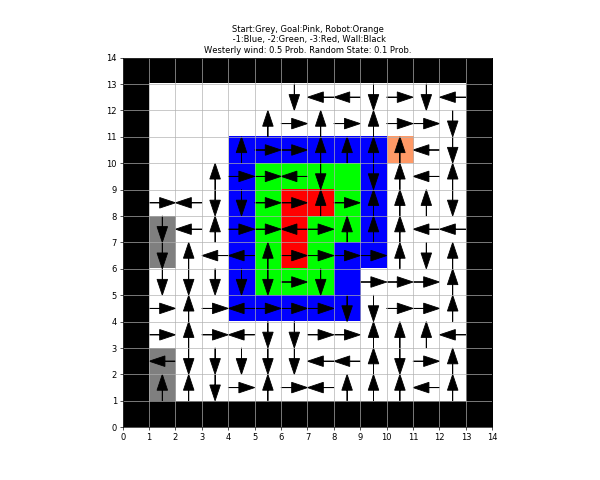
\includegraphics[width=\linewidth]{Sarsa__Problem_B_lambda_10.png}
    \caption{Sarsa lamnda(1) B }
  \end{figure}
  \centering
  \begin{figure}[b]
    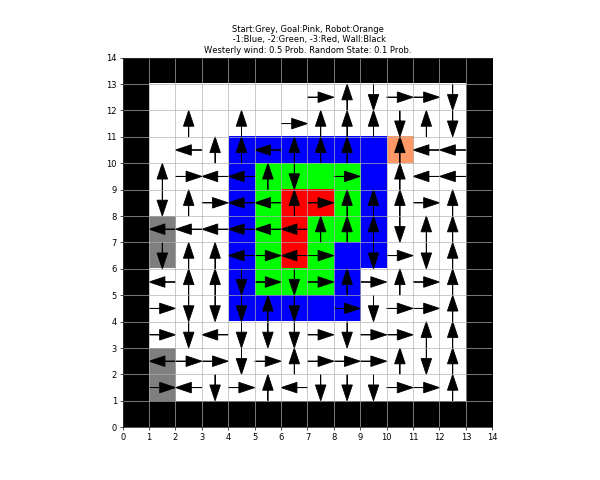
\includegraphics[width=\linewidth]{Sarsa__Problem_B_lambda_03.png}
    \caption{Sarsa lamnda(0.3) B}
  \end{figure}
  \centering
  \begin{figure}[b]
    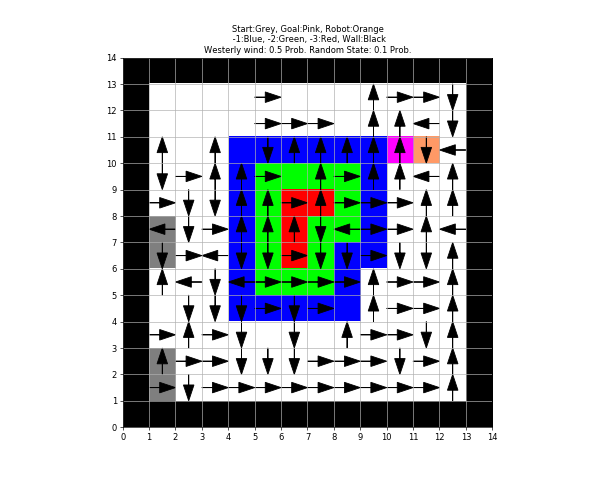
\includegraphics[width=\linewidth]{Sarsa__Problem_B_lambda_05.png}
    \caption{Sarsa lamnda(0.5) B}
  \end{figure}
  \newpage
  \centering
  \begin{figure}[b]
    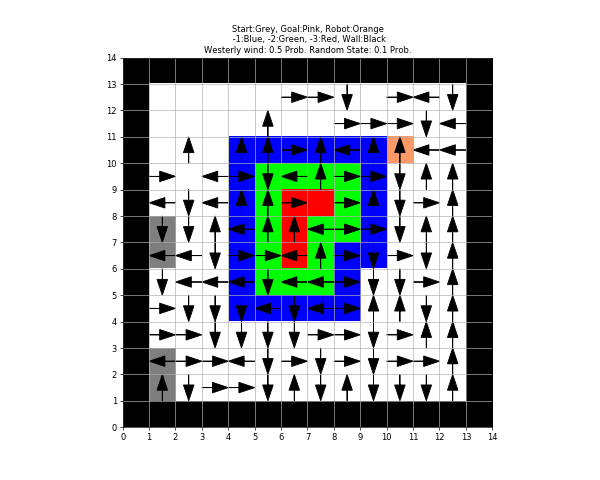
\includegraphics[width=\linewidth]{Sarsa__Problem_B_lambda_09.png}
    \caption{Sarsa lamnda(0.9) B}
  \end{figure}
  \begin{figure}[b]
    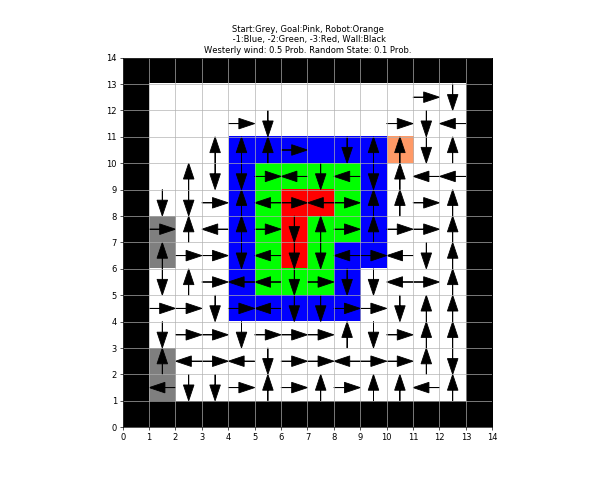
\includegraphics[width=\linewidth]{Sarsa__Problem_B_lambda_099.png}
    \caption{Sarsa lamnda(0.99) B}
  \end{figure}
  \label{fig:Softamx}


  \centering
  \begin{figure}[b]
    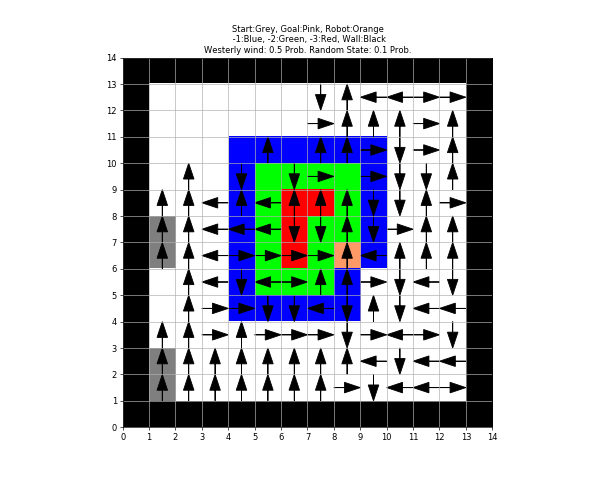
\includegraphics[width=\linewidth]{Sarsa_Problem_C_lambda_0.png}
    \caption{Sarsa lamnda(0) C }
  \end{figure}
  \centering
  \begin{figure}[b]
    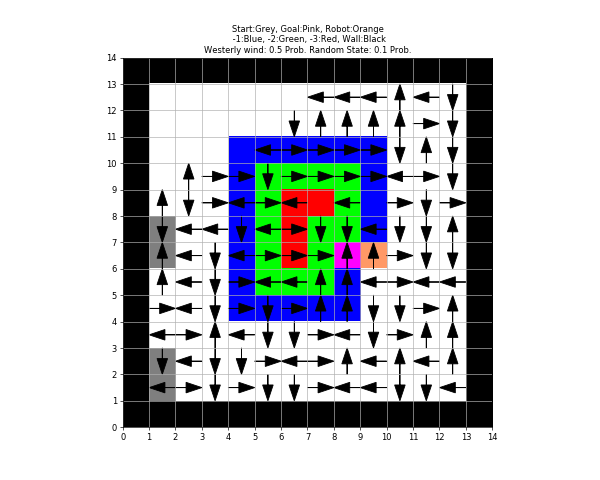
\includegraphics[width=\linewidth]{Sarsa_Problem_C_lambda_03.png}
    \caption{Sarsa lamnda(0.3) C}
  \end{figure}
  \centering
  \begin{figure}[b]
    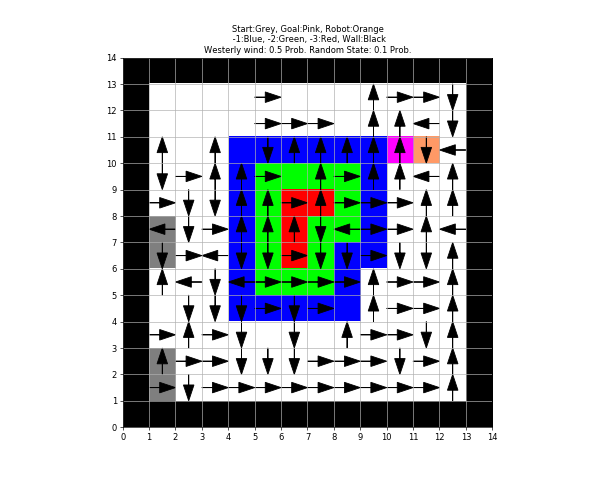
\includegraphics[width=\linewidth]{Sarsa__Problem_B_lambda_05.png}
    \caption{Sarsa lamnda(0.5) C}
  \end{figure}
  \newpage
  \centering
  \begin{figure}[b]
    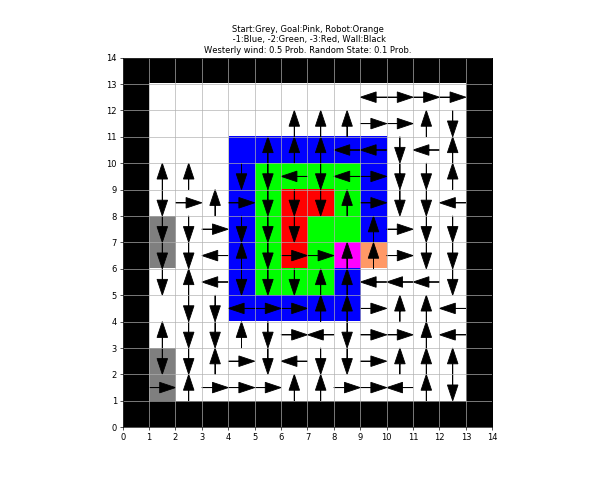
\includegraphics[width=\linewidth]{Sarsa_Problem_C_lambda_09.png}
    \caption{Sarsa lamnda(0.9) C}
  \end{figure}
  \begin{figure}[b]
    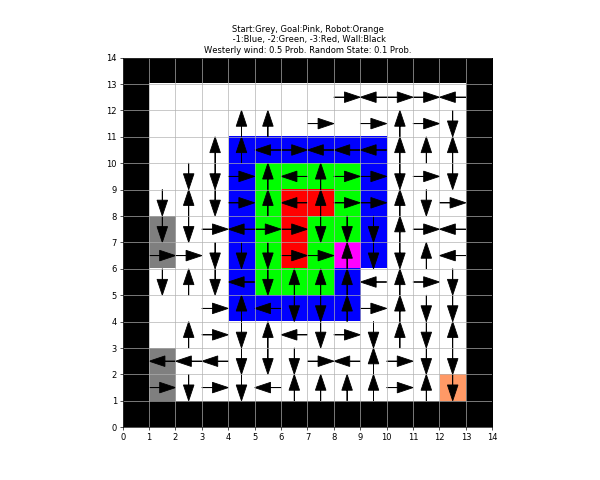
\includegraphics[width=\linewidth]{Sarsa_Problem_C_lambda_099.png}
    \caption{Sarsa lamnda(0.99) C}
  \end{figure}
  \label{fig:Softamx}

\end{document}
